\documentclass[12pt]{article}
\usepackage{hyperref}
\usepackage{graphicx}

\begin{document}

\title{CS532 Web Science - EC 0.6: Reports}
\author{Denise Legister}
\date{October 24, 2026}

\maketitle

\section{Introduction}

This report demonstrates the use of LaTeX to create a structured academic report for CS532 Web Science. It includes examples of document formatting, figures, code listings, tables, and references.

\section{Figure}
\begin{figure}[h]
\centering
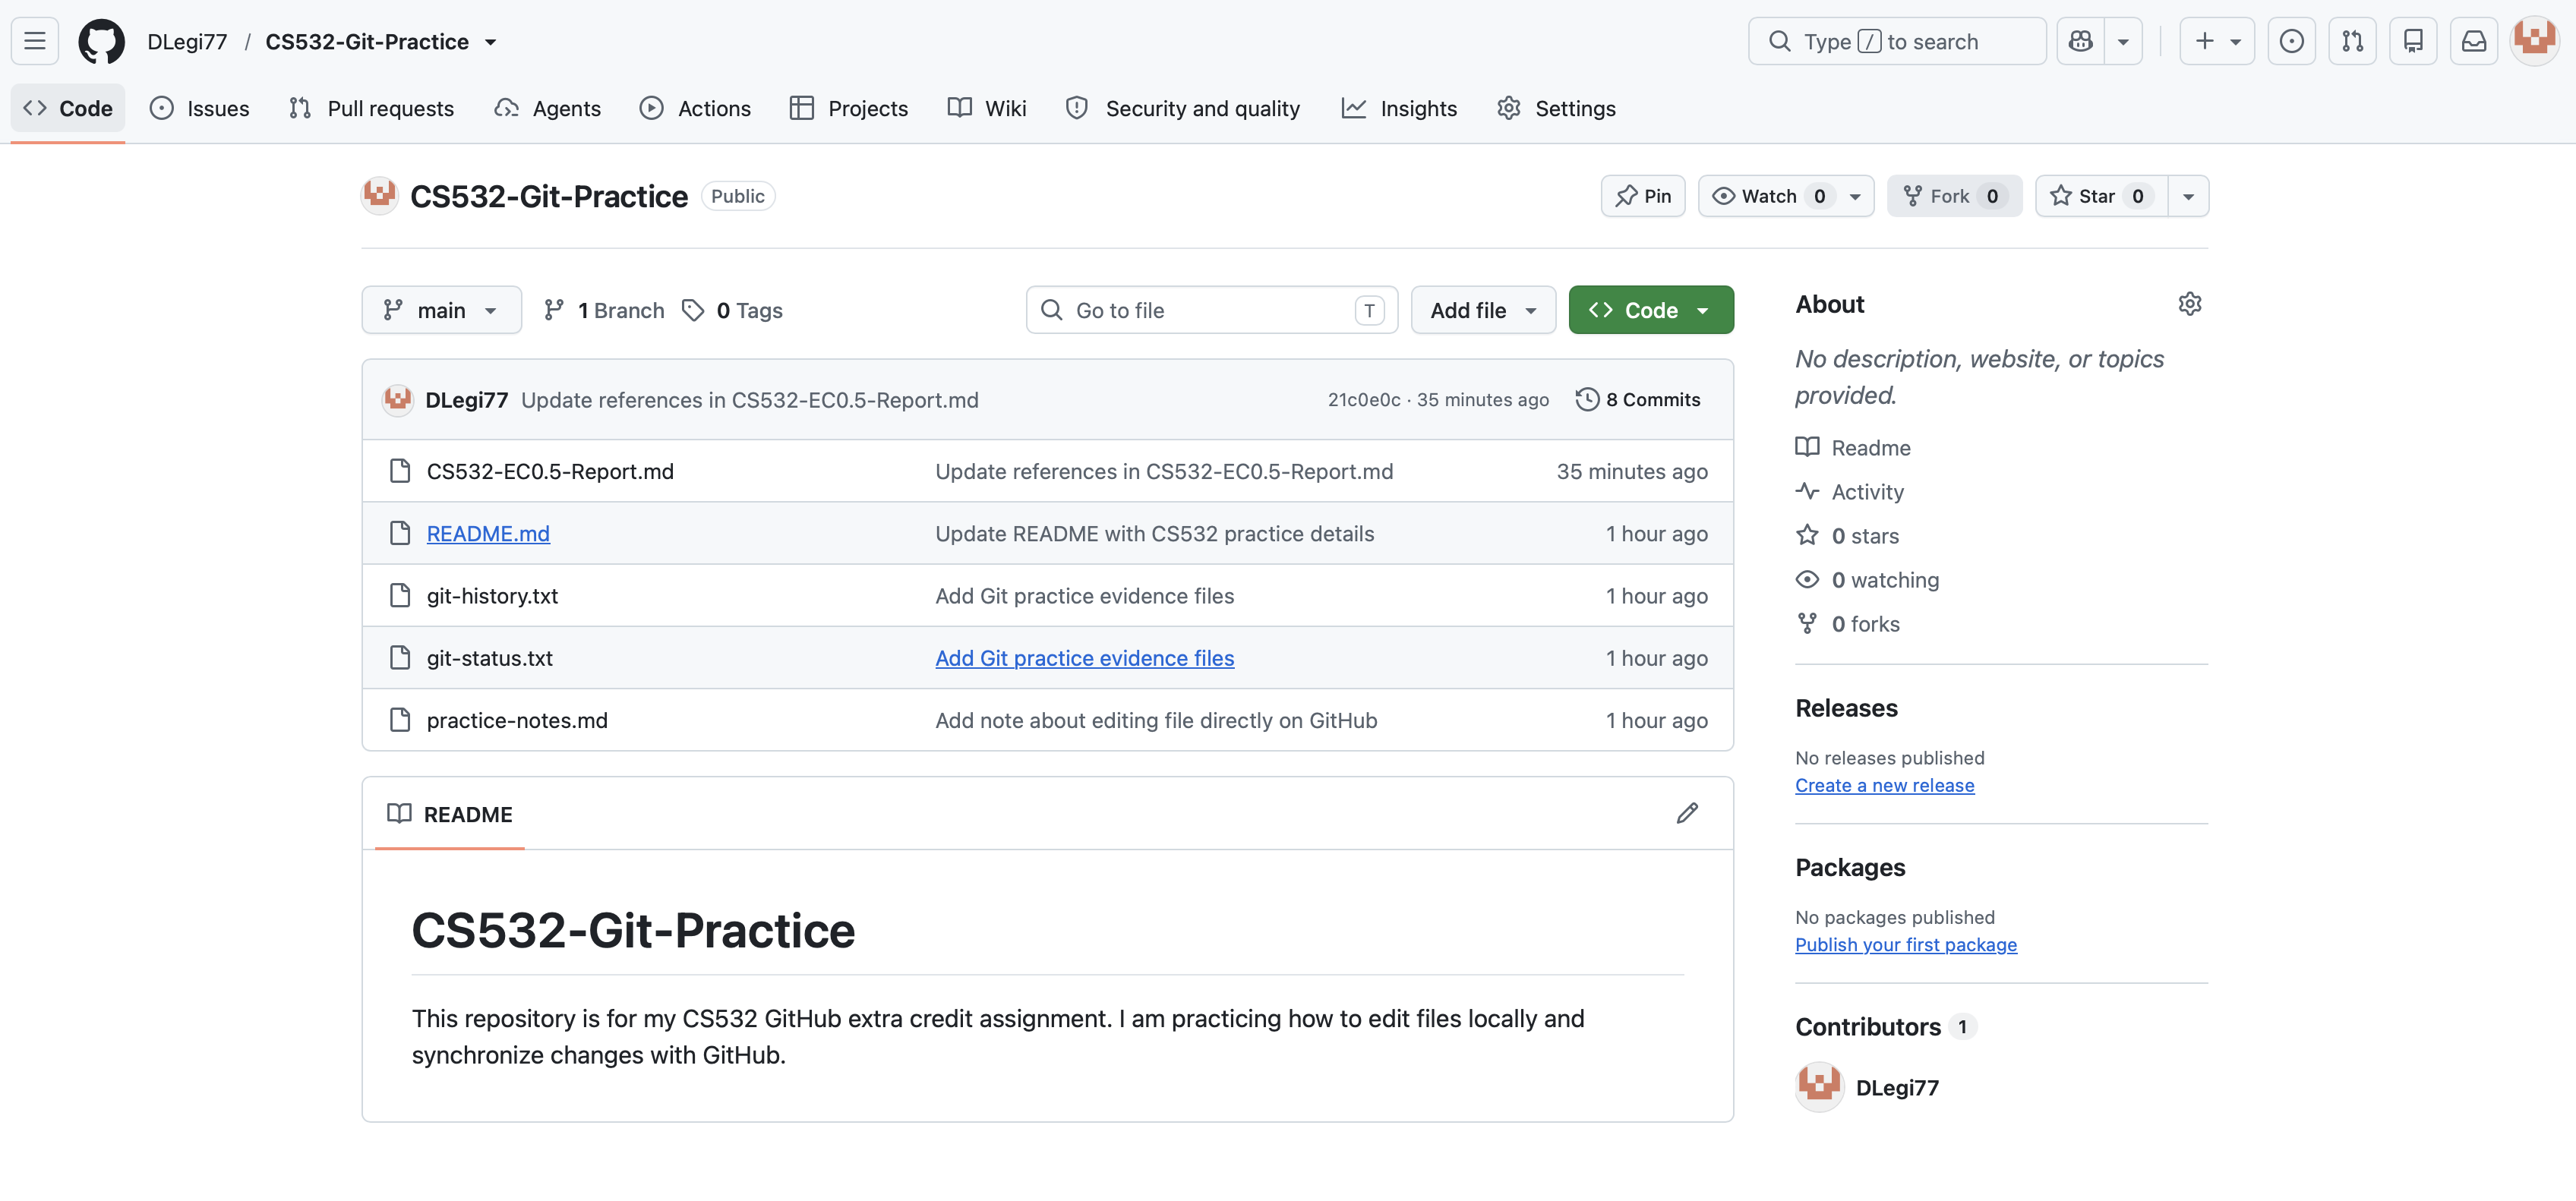
\includegraphics[width=0.8\textwidth]{github-repository.png}
\caption{GitHub repository used for the CS532 Git and GitHub extra credit assignment}
\label{fig:web}
\end{figure}

Figure~\ref{fig:web} shows the GitHub repository created for the CS532 Git and GitHub extra-credit assignment. The repository contains the files used to practice version control and document the completed work.

\section{Code Example}

The following Git commands were used to save and upload changes to my GitHub repository.

\begin{verbatim}
git add README.md
git commit -m "Update README with CS532 practice details"
git push
\end{verbatim}

\section{Table}

Table 1 summarizes the elements demonstrated in this report.

\begin{table}[h]
\centering
\begin{tabular}{|l|p{9cm}|}
\hline
Git Command & Purpose \\
\hline
git add & Stages changes for the next commit. \\
git commit & Records changes in the local repository. \\
git push & Uploads local commits to GitHub. \\
git pull & Retrieves and integrates changes from GitHub. \\
\hline
\end{tabular}
\caption{Git Commands Used and Reviewed During EC 0.5}
\label{tab:gitcommands}
\end{table}

\section{References}

The following resources were consulted:

\begin{itemize}
\item GitHub Docs. \url{https://docs.github.com/}
\item Git Documentation. \url{https://git-scm.com/docs}
\item CS532 Web Science course materials.
\end{itemize}

\end{document}